%This is my super simple Real Analysis Homework template

\documentclass{article}
\usepackage{tikz}
\usepackage{pgfplots}

\usepackage[left=.8in,right=.8in,top=1in,bottom=1in]{geometry}
\newcommand{\reals}{{\mbox{\bf R}}}
\newcommand{\dom}{{\mbox{\bf dom}}}
\newcommand{\var}{{\mbox{\bf var}}}
\newcommand{\E}{{\mbox{\bf E}}}
\newcommand{\tr}{{\mbox{\bf tr}}}
\newcommand{\prob}{{\mbox{\bf prob}}}
\newcommand{\diag}{{\mbox{\bf diag}}}
\newcommand{\rank}{{\mbox{\bf rank}}}

\usepackage[makeroom]{cancel}
\usepackage{graphicx}
\usepackage{hyperref}

\usepackage[utf8]{inputenc}
\usepackage[english]{babel}
\usepackage[]{amsthm} %lets us use \begin{proof}
\usepackage[]{amssymb} %gives us the character \varnothing
\usepackage{amsmath}
\usepackage{fancyhdr}

\pagestyle{fancy}
\fancyhf{}
\rhead{Tuguluke}
\lhead{CSCI 5254  Homework 4}
\rfoot{Page \thepage} 

\title{CSCI 5254  Homework 4}
\author{Tuguluke Abulitibu}
\date\today
%This information doesn't actually show up on your document unless you use the maketitle command below

\begin{document}
\maketitle %This command prints the title based on information entered above
\section*{Chapter 4, Basic definitions}	
\subsection*{5.1}



\subsubsection*{(a)}
\begin{itemize}
\item feasible set: $[2,4]$
\item optimal value: $x^* = 2$
\item optimal solution: $p^* = 2^2 + 1  = 5$
\end{itemize}

\subsubsection*{(b)}
    \begin{figure}[h]
\centering
\begin{minipage}{.5\textwidth}
  \centering
  \includegraphics[height=0.21\textheight,width=.8\linewidth]{51.png}
  \caption{feasible set and optimal}

\end{minipage}%
\begin{minipage}{.5\textwidth}
  \centering
  \includegraphics[height=0.21\textheight,width=.8\linewidth]{51b.png}
  \caption{with Lagrange}

\end{minipage}

\end{figure}
Lagrangian:
\[L (x, \lambda) = x^2 + 1 - \lambda(x-2)(x-4) = (1+ \lambda) x^2 -6\lambda x + 1 + 8\lambda\]
let $(-\dfrac{9\lambda^2}{1+ \lambda} + 1 + 8\lambda)' = 0$. we get $\lambda = 2$. also from Figure 2, we can easily see that lower bound property $5 = p^* \ge \inf_x L(x, \lambda)$ holds, in fact from Figure 3 we can see it hold at $\lambda =2$\\

with $ L' (x, \lambda) = 2(1 + \lambda)x - 6 \lambda = 0$, we have $x = \dfrac{3\lambda}{1+ \lambda}$
Plug back in, we get dual function
\[= (1 + \lambda) (\dfrac{3\lambda}{1+ \lambda})^2 - 6\lambda \dfrac{3\lambda}{1+ \lambda} + 1 + 8\lambda  = \dfrac{-9\lambda^2}{1+ \lambda}+ 1 + 8\lambda   \]
hence
\[g(\lambda) = \begin{cases}
           \dfrac{-9\lambda^2}{1+ \lambda}+ 1 + 8\lambda & 1+ \lambda > 0\\
          -\infty &  1+ \lambda \le 0
        \end{cases} \]
      \begin{figure}[ht]
\centering
\begin{minipage}{.5\textwidth}
  \centering
  \includegraphics[height=0.21\textheight,width=.8\linewidth]{51c.png}
  \caption{$\lambda$ plot zoom in }

\end{minipage}%
\begin{minipage}{.5\textwidth}
  \centering
  \includegraphics[height=0.21\textheight,width=.8\linewidth]{51c2.png}
  \caption{$\lambda$ plot }

\end{minipage}

\end{figure}

\subsubsection*{(c)}
By textbook definition (5.16)
    \[  \boxed{  \begin{array}{ll}
    \mbox{maximize}   &  \dfrac{-9\lambda^2}{1+ \lambda}+ 1 + 8\lambda  \\
    \mbox{subject to} & \lambda \succeq 0   
         \end{array} 
         }
  \]    
since $\nabla ( \dfrac{-9\lambda^2}{1+\lambda}\:+\:1\:+\:8\lambda) = -\dfrac{18}{\left(x+1\right)^3}$, hence it is concave.\\
From part (b), we already know $\lambda^* = 2$, and the strong duality holds.
\subsubsection*{(d)}
\begin{figure}[h]
\begin{center}
  \includegraphics[width=.4\linewidth]{51d.png}
\end{center}
\caption{ $p^*(u)$}
\end{figure}
From Figure 1 we can see that $\min f(x) =  (x-2)(x-4) = -1$, hence $p^*(u)   = -\infty$ if $u < -1$.\\
 From $x^2 -6x +8 -u = 0$, with quadratic formula, we got the solution: $x = \dfrac{6 \pm \sqrt{4 + 4u}}{2}$. Hence $[3 - \sqrt{1-u}, 3 + \sqrt{1-u}]$, we can see $x^8 = 3 - \sqrt{1-u}$
\[p^*(u)  = \begin{cases}
-\infty & u < -1 \\
x^2 + 1  = (3 - \sqrt{1-u})^2 + 1 & -1 \le u \le 8 \\
\inf( x^2 +1) = 1& u \ge 8
\end{cases}\]
Finally: 
\[\dfrac{dp}{du} = 1 - \dfrac{3}{\sqrt{1+u}} = -2 (\mbox{ when } u = 0)  = -\lambda^*\]

\section*{Chapter 4, Examples and applications}	
\subsection*{5.11}
With hint $y_i = A_i^Tx + b_i$, the problem transforms into
\[  \boxed{  \begin{array}{ll}
    \mbox{min}   &  \sum_i^N \|y_i\|_2  + \frac{1}{2}\|x - x_0\|_2^2 \\
    \mbox{subject to} & A_ix + b = y_i
         \end{array} 
         }
  \]    
  hence
\[L(x,y, \nu) = \sum_i^N \|y_i\|_2  +  \frac{1}{2}\|x - x_0\|_2^2 + \sum_i^N \nu_i^T(A_ix + b_i - y_i) \]
\[ = \underbrace{\sum_i^N \|y_i\|_2 }_{\mbox{Conjugate of a norm}}  + \underbrace{\frac{1}{2}\|x- x_0\|_2^2 + (\sum_i\nu_iA_i)x}_{\mbox{can be min by derivative}} + b^T\nu \]
since $\sum_i^N \|y_i\|_2 \begin{cases}
0, & \|y_i\|_2 \le 1\\
-\infty, & \|y_i\|_2 > 1
\end{cases}
$\footnote{Example 3.26 on page 93}, also $[\frac{1}{2}\|x- x_0\|_2^2 + (\sum_i\nu_iA_i)x]' = 0 \Rightarrow x = x_0 - \sum_i\nu_iA_i$, plug both back, we have the dual function
\[g(y_i) = \begin{cases}
 \sum_i^N \|A_i^Tx_0 + b_i\|_2  - \frac{1}{2}\|\nu_iA_i\|_2^2& \|y\| \le 1\\
-\infty, & otherwise
\end{cases}
\]
hence the dual problem: 
\[  \boxed{  \begin{array}{ll}
    \mbox{maximize}   &  \sum_i^N \|A_i^Tx_0 + b_i\|_2  - \frac{1}{2}\|A_i\nu_i\|_2^2 \\
    \mbox{subject to} & \|y_i\|_2 \le 1, \; i = 1, 2, \dots, N
         \end{array} 
         }
  \] 
\subsection*{5.13}
\subsubsection*{(a)}
\[L(x, \mu, \nu) = c^Tx + \lambda (Ax- b) - \sum_i\nu_i(x_i - x_i^2) \]
\[= c^Tx + \lambda (Ax- b) - \nu^Tx + x^T\diag(\nu)x \]
\[ = x^T\diag(\nu) x + (C + A^T\lambda - \nu)^Tx - b^T\lambda \]
by letting $L' = 2x\diag(\nu) + [C + A^T\lambda - \nu]^T = 0$, we have $x = -\dfrac{(C + A^T\lambda - \nu)^T}{2\diag(\nu)}$, plug back in, we have 
\[g(x) = \dfrac{(C + A^T\lambda - \nu)^T}{2diag(\nu)}\diag(\nu)\dfrac{(C + A^T\lambda - \nu)}{2 \diag (\nu)} - (C + A^T\lambda - \nu)\dfrac{(C + A^T \lambda - \nu)}{2 \diag(\nu)}  - b^T\lambda \]
\[ =- b^T\lambda - \frac{1}{4 \diag(\nu)}(C + A^T\mu - \nu)^2 \]
since $ \sum_i\nu_ix_i^2 = X^t \begin{bmatrix}
\nu_1 & & \\
 & \ddots& \\
 &&\nu_n
\end{bmatrix} X$ is bounded only when $\nu_i \ge 0, \, \forall i $, then
we get  the dual function
\[g(\lambda, \nu) = \begin{cases}
- b^T\lambda - \frac{1}{4 }\sum_i \dfrac{(c_i + a_i^T\lambda_i - \nu_i)^2}{\nu_i} & \nu \ge 0 \\
-\infty& \mbox{ Otherwise}
\end{cases}
\]
Dual problem 
 \[  \boxed{  \begin{array}{ll}
    \mbox{maximize}   &   -b^T\lambda - \frac{1}{4 }\sum_i \dfrac{(c_i + a_i^T\lambda_i - \nu_i)^2}{\nu_i} \\
    \mbox{subject to} & \nu \succeq 0   
         \end{array} 
         }
  \]    
  Since $\sup_{\nu_i} - \dfrac{(c_i + a_i^T\lambda_i - \nu_i)^2}{\nu_i}\ \begin{cases}
  c_i + a_i^T\lambda_i  & c_i + a_i^T\lambda_i  \le 0\\
  0 & c_i + a_i^T\lambda_i > 0
  \end{cases}
  $, therefore we can rewrite the problem as: 
\[
  \boxed{  \begin{array}{ll}
    \mbox{maximize}   &   -b^T\lambda + \sum_i \min \{0, (c_i + a_i^T\lambda_i) \}\\
    \mbox{subject to} & \lambda \succeq 0   
         \end{array} 
         }
\]
  Which will come in handy in part (b)
\subsubsection*{(b)}
Let us copy the LP-relaxation, and since \[
0 \le x_i \le 1 \leftrightarrow \begin{cases}
-x_i \le 0 \\
x_i -1 \le 0
\end{cases}
\]

therefore\footnote{ ${\bf 1} = [1,1, \dots, 1]^T$}
\[L = c^T + \mu^T(Ax-b) - \nu^Tx + w^T(x -  {\bf 1)}\]
which is linear (bounded when coefficient of x is zero), hence we have 
\[g(\mu,\nu,w) = \begin{cases}
-\mu^Tb -w^T{\bf 1}; & c+ A^T\mu-\nu + w = 0\\
-\infty ; & otherwise
\end{cases}
\]
convert it into dual problem:
  \[  \boxed{  \begin{array}{ll}
    \mbox{maximize}   &   -b^T\mu -{\bf 1}^Tw \\
    \mbox{subject to} &c+ A^T\mu-\nu + w = 0 \\
    & \mu, \nu, w \succeq 0  
         \end{array} 
         }
  \]   
  let $\nu = 0 $: 
  \[  \boxed{  \begin{array}{ll}
    \mbox{maximize}_{\mu, w}   &   -b^T\mu -{\bf 1}^Tw \\
    \mbox{subject to} &c+ A^T\mu + w = 0 \\
    & \mu, w \succeq 0  
         \end{array} 
         }
  \]   
  further, we make it into solve for $w$:
  \[  \boxed{  \begin{array}{ll}
    \mbox{maximize}_{ w}   &   -b^T\mu -{\bf 1}^Tw \\
    \mbox{subject to} &c+ A^T\mu + w = 0 \\
    &  w \succeq 0  
         \end{array} 
         }
  \]
 Here we can see this is the same as part(a), hence {\bf the lower bound obtained via lagrangian relaxation and via the LP relaxation are the same}. 
  
\section*{Chapter 4, Optimality conditions}	
\subsection*{5.26}

\subsubsection*{(a)}
\begin{center}

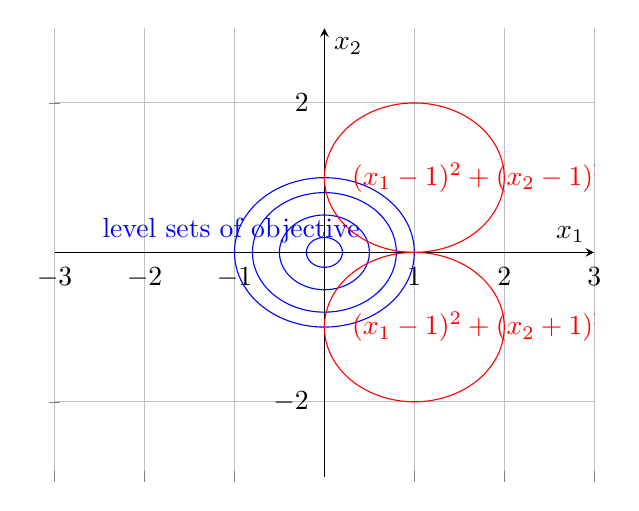
\begin{tikzpicture} 
  \begin{axis}  [
        xlabel={$x_1$}, 
        ylabel={$x_2$},
        xmin = -3,
        xmax = 3,
        ymin = -3,
        ymax = 3,
        grid=both,
        axis lines=middle,
        tick pos = left,
      ]  \addplot [domain=-180:180, samples=100, color=blue] ({cos(x)},{sin(x)});
    \addplot [domain=-180:180, samples=100, color=blue] ({.5*cos(x)},{.5*sin(x)})
    node [pos=0.5, above left] {level sets of objective};
    \addplot [domain=-180:180, samples=100, color=blue] ({.8*cos(x)},{.8*sin(x)});
    \addplot [domain=-180:180, samples=100, color=blue] ({.2*cos(x)},{.2*sin(x)});

    \addplot [domain=-180:180, samples=100, color=red] ({cos(x)+1},{sin(x)- 1})
    node [pos=0.5] {$(x_1 -1)^2 + (x_2+1)^2 \le 1$};
    \addplot [domain=-180:180, samples=100, color=red] ({cos(x)+1},{sin(x)+ 1})
node [pos=0.5] {$(x_1 -1)^2 + (x_2-1)^2 \le 1$};

   \end{axis}
\end{tikzpicture}
\end{center}
$x^* = (1,0)$, and $p^* = 0^2 + 1^2 =  1$
\subsubsection*{(b)}
\begin{itemize}
\item primal feasibility: $ \begin{cases}
(x_1 -1)^2 + (x_2-1)^2 \le 1 \\
(x_1 -1)^2 + (x_2+1)^2 \le 1
\end{cases} $
\item dual feasibility : $ \begin{cases}
\lambda_1 \ge 0 \\
\lambda_2 \ge 0 
\end{cases} $
\item complimentary slackness: $ \begin{cases}
\lambda_1 [(x_1 -1)^2 + (x_2 -1)^2 -1] = 0 \\
\lambda_2[(x_1 -1)^2 + (x_2 +1)^2 -1] = 0
\end{cases} $
\item first order condition:  $ \begin{cases}
2x_1 + 2(x_1 -1)\lambda_1 +  2(x_1 -1)\lambda_2= 0 \\
2x_2 + 2(x_2 -1)\lambda_1 +  2(x_2 +1)\lambda_2= 0 \\

\end{cases} $
\end{itemize}
plug $x^* = (1,0)$ into KKT, we have 
\[\begin{cases}
1 \le 1 \\
\lambda_{1,2} \ge 0\\
2 = 0\\
0= 0\\
-2\lambda_1 + 2\lambda_2 = 0
\end{cases}
\]
the dual optimal is not obtained, which just show that there {\bf does not exist $\lambda_1^*, \lambda_2^*$ that $x^*$ is optimal. }
\subsubsection*{(c)}
\[L(x_1, x_2,\lambda_1, \lambda_2) = x_1^2 + x_2^2 + \lambda_1 [(x_1 -1)^2 + (x_2 -1)^2 -1] + \lambda_2[(x_1 -1)^2 + (x_2 +1)^2 -1] \]
\[L(x_1, x_2,\lambda_1, \lambda_2) = x_1^2 + x_2^2 + \lambda_1 [(x_1^2 -2x_1 +1) + (x_2^2 -2x_2  +1) -1] + \lambda_2[(x_1 ^2-x_1+1) + (x_2^2 + 2x_2 +1) -1] \]
\[ = (1+ \lambda_1 + \lambda_2)x_1 -2(\lambda_1 + \lambda_2)x_1+ (1+ \lambda_1 + \lambda_2)x_2  -2(\lambda_1 -\lambda_2)x_2 + \lambda_1 + \lambda_2\]
by letting \[
\begin{cases}
\dfrac{\partial L}{\partial x_1} =2x_1(1+ \lambda_1 + \lambda_2)-2(\lambda_1 +\lambda_2)= 0\\
\dfrac{\partial L}{\partial x_1} =2x_2(1+ \lambda_1 + \lambda_2)-2(\lambda_1 -\lambda_2)= 0
\end{cases}
\]
we get $x^* = (\dfrac{\lambda_1 +\lambda_2}{1+ \lambda_1 + \lambda_2} ,\dfrac{\lambda_1 -\lambda_2}{1+ \lambda_1 + \lambda_2} )$, plug back in, we will get dual function
\[g(\lambda_1, \lambda_2) = 
\begin{cases}
\dfrac{-2(\lambda_1 -\lambda_2)^2 - 2(\lambda_1 -\lambda_2)^2}{1+ \lambda_1 + \lambda_2} + \lambda_1 + \lambda_2 & 1+ \lambda_1 + \lambda_2 \ge 0 \\
-\infty & otherwise
\end{cases}
\]
simplify further 
\[\dfrac{-2(\lambda_1 -\lambda_2)^2 - 2(\lambda_1 -\lambda_2)^2}{1+ \lambda_1 + \lambda_2} + \lambda_1 + \lambda_2 = 
\dfrac{\lambda_1 + \lambda_2 + 2 \lambda_1\lambda_2 - \lambda_1^2 -\lambda_2^2}{1+ \lambda_1 +\lambda_2}\]
we can rewrite the Lagrange dual problem as 
 \[  \boxed{  \begin{array}{ll}
    \mbox{maximize}   &   \dfrac{\lambda_1 + \lambda_2 + 2 \lambda_1\lambda_2 - \lambda_1^2 -\lambda_2^2}{1+ \lambda_1 +\lambda_2}\\
    \mbox{subject to} & \lambda_1, \lambda_2 \ge 0
             \end{array} 
         }
  \]
this dual is a limit, also it does not satisfy slater condition, from part (b) that KKT has no solution, hence the dual-optimal is not attained.
\subsection*{5.27}
\begin{itemize}
\item primal feasibility $Gx - h \le 0$
\item dual feasibility $\nu \ge 0$
\item complimentary slackness $\nu(Gx - h) = 0$
\item first order condition:  $ 2xA^TA + G\nu^T - 2A^Tb  + \nu G = 0$
\end{itemize}
now we work on Lagrange: 
\[L(x,\nu) = (Ax - b)^T(Ax - b) + \nu^T(GX-h) = (x^TA^T - b^T)(Ax - b) + \nu^T(GX-h)\]
 \[ = x^TA^TAx - bx^TA^T -b^TAx - b^Tb + \nu^TGx - \nu^Th\]
 \[ = x^TA^TAx + (\nu^TG-2bA^T )x + b^Tb -\nu^Th\]
by letting  $L' =  (x^TA^TAx + (\nu^TG-2bA^T )x + b^Tb -\nu^Th)' = 2xA^TA + G\nu^T - 2A^Tb = 0 $, \\
we get \[x^* = \dfrac{2A^Tb - G^T\nu}{2A^TA} \] plug back in feasibility $Gx - h = 0$, we get
\[v^* = \dfrac{G2A^Tb - 2A^Ah}{GG^T}\]
Hence 
\[x^* = \dfrac{2A^Tb - G^T\frac{G2A^Tb - 2A^Ah}{GG^T}}{2A^TA}  =\dfrac{2A^Tb - 2A^Tb - 2A^AG^{-1}h}{2A^TA} \] 
\section*{Generalized inequalities}	
\subsection*{5.39}
\subsubsection*{(a)}
The solution is at ${\bf rank} X = 1$, hence $x_{ij} = x_ix_j \Leftrightarrow X = xx^T$, also for for scalar, inner product/trace can be written as $\tr (WX) = \tr (W xx^T) = \tr ( x^TWx)  =  x^TWx$, finally $X_{ii} = (xx^T)_{ii} = x_i^2 $.\\
Hence the two are the same
\subsubsection*{(b)}
\[\begin{array}{ll}
    \mbox{minimize}   &  \tr (WX)\\
    \mbox{subject to} & X_{ii} =1, \, \forall i \\
    & \rank X = 1
             \end{array} \]
      here since the rank is non-convex, we need to drop the $\rank$ function, this 'reduction' along show that {\bf relaxation gives a lower bound on the optimal value of TW partitioning}.\\
      {\bf $X^*$ is optimal if rank X is 1}
\subsubsection*{(c)}
Show the Lagrange dual of one problem is the other, since dual gives you the lower bound.
\[\boxed{ \begin{array}{ll}
    \mbox{maximize}   &  -{\bf 1}^T\nu\\
    \mbox{subject to} & W + \diag(\nu) \succeq 0
             \end{array}    \Longleftrightarrow \begin{array}{ll}
    \mbox{minimize}   &  {\bf 1}^T\nu\\
    \mbox{subject to} & W + \diag(\nu) \succeq 0
             \end{array} }\]
             \[L = {\bf 1}^T \nu -\tr (X(W + \diag(\nu))) = -\tr (XW) + \sum_i (\nu_i - \nu_iX_{ii}) = -\tr (WX) + \sum_i (\nu_i - \nu_iX_{ii})  \]
           here $  \sum_i (\nu_i - \nu_iX_{ii}) $ is a linear function of $\nu$, so the coefficient $(1 - X_{ii})$ has to be zero in order to for the problem to be bounded, therefore $X_{ii} =1$, hence the dual problem: 
\[\boxed{
\begin{array}{ll}
    \mbox{maximize}   &  -\tr (WX)\\
    \mbox{subject to}  &X \succeq 1 \\
    & X_{ii}  = 1 \: \forall i 
             \end{array}    \Longleftrightarrow \begin{array}{ll}
    \mbox{minimize}   &  \tr (WX)\\
  \mbox{subject to} & X \succeq 1 \\
    & X_{ii} = 1 \; \forall i 
             \end{array} }\]
We showed (5.114) and (5.115) has same lower bound.

 \section*{Additional }
 \subsection*{3.3}
\subsubsection*{(a)}
since $\begin{cases}
\|x + 2y\| = 0\\
\|x - y\| = 0\\
\end{cases} = 
\begin{cases}
x = 0\\
y= 0\\
\end{cases}
$
so 
\begin{verbatim}
[x + 2*y == 0, x - y == 0]
\end{verbatim}

\subsubsection*{(b)}
syntax error:
\begin{verbatim}
[square(x + y) <= u, square(u) <= x-y]
\end{verbatim}

\subsubsection*{(c)}
syntax error:
\begin{verbatim}
[inv_pos(x) + inv_pos(y) <=1]
\end{verbatim}
\subsubsection*{(d)}
syntax error:
\begin{verbatim}
[norm(hstack([u,v])) <= 3*x + y, maximum(x, 1) <= u, maximum(y,2) <=v]\end{verbatim}
\subsubsection*{(e)}
syntax error:
\begin{verbatim}
[quad_over_lin(x+y, sqrt(y)) <= x -y +5]
\end{verbatim}
\subsubsection*{(f)}
syntax error:
\begin{verbatim}
[x >= inv_pos(y)]
\end{verbatim}
\subsubsection*{(g)}
syntax error:
\begin{verbatim}
[quad_over_lin(square(x),x) + quad_over_lin(square(y),y) <= 1]
\end{verbatim}

\subsubsection*{(h)}
\begin{verbatim}
import numpy as np
import cvxpy as cp

x = cp.Variable()
y = cp.Variable()
u = cp.Variable()
v = cp.Variable()

v_1 = np.random.randint(10, size = 10000)
v_2 = np.random.randint(10, size = 10000)
v_3 = np.random.randint(10, size = 10000)
v_4 = np.random.randint(10, size = 10000)

# constraints = [x + 2*y == 0, x - y == 0]
# constraints = [square(x + y) <= u, square(u) <= x-y]
# constraints = [inv_pos(x) + inv_pos(y) <=1]
# constraints = [norm(hstack([u,v])) <= 3*x + y, maximum(x, 1) <= u, maximum(y,2) <=v]
# constraints = [quad_over_lin(x+y, sqrt(y)) <= x -y +5]
# constraints = [x >= inv_pos(y)]
constraints  = [quad_over_lin(square(x),x) + quad_over_lin(square(y),y) <= 1]

objective = cp.Minimize(cp.sum(cp.abs(v_1 - (v_2 * x + v_3 * y + v_4 * z))))

prob = cp.Problem(objective, constraints)
print("Value of OF:", prob.solve())
print('Current value of controls:')
print(x.value, y.value)
\end{verbatim}

\end{document}